\documentclass[a5paper,titlepage,10pt,openany]{scrbook}
\usepackage[a5paper,backref]{hyperref}
\usepackage[papersize={148.5mm,215mm},twoside,bindingoffset=0.5cm,hmargin={2cm,2cm},
				vmargin={2cm,2cm},footskip=1.1cm,driver=dvipdfm]{geometry}
\usepackage{palatino}
\usepackage{pstricks}
\usepackage{graphicx}
\usepackage[bahasa]{babel} 
%\usepackage[pdftex]{dropping}
\usepackage{lettrine}
\usepackage{pifont}
\usepackage{enumitem}
\usepackage{wrapfig}
\usepackage{indentfirst}

\author{Lingkungan St. Petrus Maguwo}
\title{Warta Iman}
\setlength{\parindent}{1cm}
\psset{unit=1mm}

\makeatletter
\renewcommand{\@makeschapterhead}[1]{%
  {\parindent \z@ \centering \normalfont
    \interlinepenalty\@M \Large \bfseries #1\par\nobreak \vskip 20\p@ }}
\renewcommand{\section}{\@startsection {section}{1}{\z@}%
                                   {-3.5ex \@plus -1ex \@minus -.2ex}%
                                   {2.3ex \@plus.2ex}%
%                                   {\normalfont\normalsize\bfseries\centering}}
                                   {\normalfont\normalsize\bfseries}}
\renewcommand\subsection{\@startsection{subsection}{2}{\z@}%
                                     {-3.25ex\@plus -1ex \@minus -.2ex}%
                                     {1.5ex \@plus .2ex}%
                                     {\normalfont\normalsize\bfseries}}
\renewcommand\subsubsection{\@startsection{subsubsection}{3}{\parindent}%
                                    {3.25ex \@plus1ex \@minus.2ex}%
                                    {-1em}%
                                    {\normalfont\normalsize\bfseries}}

\makeatother

\makeatletter  % Allow the use of @ in command names
\long\def\@makecaption#1#2{%
  \vskip\abovecaptionskip
  \sbox\@tempboxa{{#1#2}}%
  \ifdim \wd\@tempboxa >\hsize
    {#1#2\par}
  \else
    \hbox to\hsize{\hfil\box\@tempboxa\hfil}%
  \fi
  \vskip\belowcaptionskip}
\makeatother   % Cancel the effect of \makeatletter

\newcommand{\chap}[1]{%
    \chapter*{#1}
	\addcontentsline{toc}{chapter}{#1}
    }

\newcommand{\sumber}[1]{%    
	\begin{flushright}
	{\emph{#1}}
	\end{flushright}
}
\newcommand{\qti}[1]{%    
	\begin{quote}
	{\emph{#1}}
	\end{quote}
}

\hyphenation{sa-u-da-ra-ku}
\hyphenation{ke-ri-ngat}
\hyphenation{je-ri-tan}
\hyphenation{hu-bung-an}
\hyphenation{me-nya-dari}
\hyphenation{Eng-kau}
\hyphenation{ke-sa-lah-an}
\hyphenation{ba-gai-ma-na}
\hyphenation{Tu-han}
\hyphenation{di-per-ca-ya-kan}
\hyphenation{men-ja-uh-kan}
\hyphenation{bu-kan-lah}
\hyphenation{per-sa-tu-kan-lah}
\hyphenation{ma-khluk}
\hyphenation{Sem-buh-kan-lah}
\hyphenation{ja-lan}
\hyphenation{mem-bu-tuh-kan}
\hyphenation{be-ri-kan-lah}
\hyphenation{me-ra-sa-kan}
\hyphenation{te-man-ilah}
\hyphenation{mem-bi-ngung-kan}
\hyphenation{di-ka-gum-i}
\hyphenation{ta-ngis-an-Mu}
\hyphenation{mi-lik-ilah}

\renewcommand{\figurename}{~}
\renewcommand\thefigure{~}

\setlength{\itemsep}{0cm}

\begin{document}
\pagestyle{plain}
\thispagestyle{empty}
\newcommand{\edisi}[1]{%
\DeclareFixedFont{\PT}{T1}{ppl}{b}{}{0.7in}
\DeclareFixedFont{\PTit}{T1}{ppl}{b}{it}{0.7in}
\DeclareFixedFont{\PTsmall}{T1}{ppl}{b}{it}{0.25in}
\DeclareFixedFont{\PTsmaller}{T1}{ppl}{b}{it}{0.175in}
\DeclareFixedFont{\PTsmallest}{T1}{ppl}{b}{it}{0.15in}

\begin{pspicture}(14cm,2cm)
\rput[rb](10.35cm,3cm){\PTsmallest {#1}}
\rput[lb](-2cm,1.5cm){\PT {WARTA IMAN}}
\rput[lb](0cm,0.5cm){\PTsmall {Lingkungan St. Petrus Maguwo}}
\end{pspicture}%
}

\newcounter{kgkcounter}[chapter]
\renewcommand{\thekgkcounter}{\arabic{kgkcounter}. }
\newcommand{\kgk}[1]{\refstepcounter{kgkcounter}\textbf{\flushleft \textbf{\thekgkcounter #1}}\\}

\newcommand{\kutipan}[1]{%
\noindent{\framebox{\parbox{10cm}{\centering\emph{#1}}}}}

\edisi{November 2011}

%\vspace{1cm}

\begin{center}
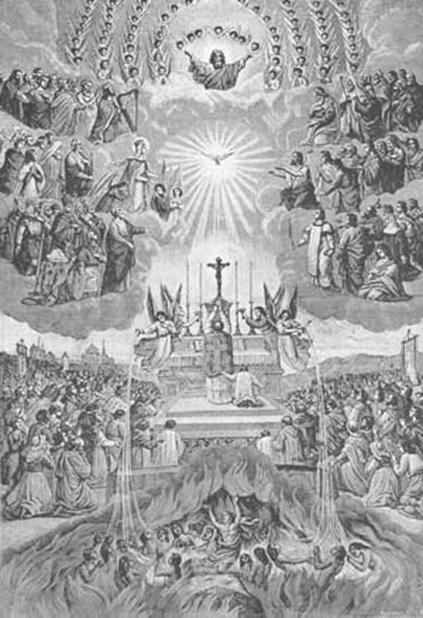
\includegraphics[scale=0.85]{gambar/purgatory2.jpg}
\end{center}

%\vspace{1cm}

\begin{center}
{\PTsmaller {Kasih, kerendahan hati, dan menurut pada kehendak Allah }}
\end{center}

\newpage

\chapter*{Dari Redaksi}
\footnotesize
\indent{Berkah Dalem,}
Bulan Maret sudah memasuki masa Prapaskah. Tidak ada salahnya jika kita mengambil tema \textit{Prapaskah} untuk edisi kali ini. Mungkin kita masih bertanya-tanya kenapa setiap masa prapaskah kita berpuasa dan berpantang. Bagian awal WI edisi kali mencoba menjawab pertanyaan tersebut.

\bigskip
Menjelang prapaskah kita sudah mendengar pembacaan pesan Bapa Uskup dalam menyongsong masa prapaskah. Dalam edisi ini Anda dapat menyimak pesan dari Bapa Paus Benediktus dalam rangka menyongsong Prapaskah 2012.

\bigskip
Masa prapaskah diawali dengan hari Rabu Abu. Kenapa Rabu dan kenapa abu? Juga kenapa digunakan daun palm bukan yang lain? Jawabannya dapat Anda simak dalam edisi kali ini. 
 
\bigskip
Renungan tentang 4 prinsip hidup dan ketika garam kehilangan asinnya melengkapi edisi kali ini. Kutipan Kompendium Gereja Katolik masih berlanjut sampai pada nomor 30 -- 33.

\bigskip

Warta lingkungan kali ini tidak memuat pasangan yang berulangtahun, karena data yang ada redaksi tidak ditemukan warga St. Petrus yang berulangtahun perkawinan bulan Maret. Redaksi tetap berharap partisipasi umat untuk meramaikan rubrik ini dengan mengirim sms berupa saran, kritik, pertanyaan, atau sekedar \textit{uneg-uneg}, dengan harapan terjalin komunikasi antar umat dan juga pengurus. Tema bulan April adalah Paskah sedang bulan Mei adalah Liturgi. Sekali lagi ditunggu partisipasi seluruh umat.
\normalsize

\begin{center}***\end{center} 

\vfill

\noindent{\framebox{\parbox{10cm}{\small
Warta Iman\\
Media komunikasi dan informasi umat lingkungan St. Petrus\\
Alamat Redaksi: Lingkungan St. Petrus Maguwo\\
E-mail: stpetrusmgw@gmail.com
}}}
\normalsize


\tableofcontents
\chap{Adven: Momen Membangun Harapan}
\small

\section*{Pengertian Adven} 

Adven berasal dari bahasa Latin, \textit{adventus}, yang artinya kedatangan. Orang Katolik Perancis pada awalnya memakai kata \textit{adventus} untuk menamakan masa persiapan menyambut Hari Raya Epifani dimana para calon baptis dibaptis menjadi warga Gereja. Gereja Katolik kemudian memakai kata \textit{adventus} untuk menamakan masa persiapan perayaan Kelahiran Yesus Kristus, yaitu Hari Raya Natal. Masa Adven berlangsung selama 4 minggu, dimulai hari minggu dan biasanya setelah tanggal 26 November. Masa Adven mempunyai 2 tujuan utama, yaitu

\begin{enumerate}[itemsep=0ex]
\item mengarahkan hati, supaya dengan penuh harapan kita menantikan kedatangan Tuhan Yesus yang kedua pada akhir zaman.
\item menyiapkan Hari Natal, memperingati kedatangan Tuhan Yesus yang pertama dulu, di Betlehem, dengan kata lain mempersiapkan kedatangan Yesus Kristus secara Sakramental pada hari Natal.
\end{enumerate}

Katekismus Gereja Katolik menekankan makna ganda ``kedatangan'' ini: ``Dalam perayaan liturgi Adven, Gereja menyongsong kedatangan Mesias; dengan demikian umat beriman mengambil bagian dalam persiapan yang lama menjelang kedatangan pertama Penebus dan membaharui di dalamnya kerinduan akan kedatangan-Nya yang kedua.'' Jadi makna adven untuk kita: bersiap-siap dan berjaga-jaga setiap saat dalam menantikan kedatangan Tuhan Yesus. Hakikat adven adalah persiapan diri. Persiapan diri yang seperti apakah itu, yaitu tindakan yang selalu berjaga-jaga (awareness), dan menyiapkan hati, dengan
\textbf{bertobat,
berdoa,} dan \textbf{
berbuat amal kasih
}

Oleh sebab itu, di satu pihak, umat beriman merefleksikan kembali dan didorong untuk merayakan kedatangan Kristus yang pertama ke dalam dunia ini. Kita merenungkan kembali misteri inkarnasi yang agung ketika Kristus merendahkan diri, mengambil rupa manusia, dan masuk dalam dimensi ruang dan waktu guna membebaskan kita dari dosa. Di lain pihak, kita  ingat dalam Syahadat bahwa Kristus akan datang kembali untuk mengadili orang yang hidup dan mati dan kita harus siap untuk bertemu dengannya. 

Adventus ini pada hakikatnya adalah seperti dalam injil, tentang perumpamaan dalam injil Matius, tentang 5 orang gadis bodoh dan 5 gadis pandai. Gadis-gadis pandai yang selain membawa pelitanya, mereka juga membawa bekal berupa minyak. Karena kita tidak tahu, akan hari maupun saatnya kan tiba. Jadi di masa adven inilah kita harus seperti gadis-gadis yang membawa bekal minyak. 

Kita memang harus selalu siap secara batiniah dalam menyambut kedatangan/kelahiran penebus kita. Apabila di dalam Injil membahasakan persiapan tersebut sebagai ``bekal'' minyak lentera yang penuh, nah, di dalam kehidupan kita secara nyata, ''bekal'' tersebut adalah: persiapan kita, dalam bentuk: bertobat, berdoa, dan beramal kasih. Nah, Masa persiapan ini berlangsung selama 4 minggu, kita biasa sebut sebagai 4 minggu persiapan. Meskipun minggu terakhir Adven pada umumnya terpotong dengan tibanya Hari Natal. Namun untuk adven kali ini, pas sekali, utuh, karena Hari Natal kita, jatuh di hari minggu. 

\section*{Lingkaran Adven}

\begin{wrapfigure}{l}{4cm}
\centering

\includegraphics[scale=0.35]{gambar/advent4.png}
\end{wrapfigure}


\noindent{Pada masa adven, di gereja ada empat batang lilin, 3 yang berwarna ungu dan 1 berwarna merah muda. Dan diikat dengan lingkaran daun2 berwarna hijau. 
Warna ungu melambangkan Pertobatan, Adven adalah masa di mana kita mempersiapkan jiwa kita untuk menyambut kedatangan Kristus pada Hari Natal. Korona/lingkaran Adven, selalu dibuat dari daun-daun \textit{evergreen}. Dahan-dahan \textit{evergreen}, sama seperti namanya ``\textit{ever green}'' – senantiasa hijau, senantiasa hidup. \textit{Evergreen} melambangkan
\textbf{Pengharapan}, \textbf{Kehidupan}, itulah Kristus, yang mati namun hidup kembali untuk selamanya.
\textbf{Keabadian jiwa kita}. Kristus datang ke dunia untuk memberikan kehidupan yang tanpa akhir bagi kita.}

Tampak tersembul di antara daun-daun \textit{evergreen} yang hijau adalah buah-buah \textit{berry} warna merah. Buah-buah itu serupa tetesan-tetesan darah, lambang darah yang dicurahkan oleh Kristus demi umat manusia. Buah merah itu mengingatkan kita bahwa Kristus datang ke dunia untuk wafat bagi kita dan dengan demikian menebus kita. Oleh karena Darah-Nya yang tercurah itu, kita beroleh hidup yang kekal. Empat batang lilin diletakkan sekeliling Lingkaran Adven, tiga lilin berwarna ungu dan yang lain berwarna merah muda. Lilin-lilin itu melambangkan keempat minggu dalam Masa Adven, yaitu masa persiapan kita menyambut Natal. Setiap hari, dalam bacaan Liturgi Perjanjian Lama dikisahkan tentang penantian bangsa Yahudi akan datangnya Sang Mesias, sementara dalam Perjanjian Baru mulai diperkenalkan tokoh-tokoh yang berperan dalam Kisah Natal. Pada awal Masa Adven, sebatang lilin dinyalakan, kemudian setiap minggu berikutnya lilin lain mulai dinyalakan. Seiring dengan bertambah terangnya Lingkaran Adven setiap minggu dengan bertambah banyaknya lilin yang dinyalakan, kita pun diingatkan bahwa kelahiran Sang Terang Dunia semakin dekat. Semoga jiwa kita juga semakin menyala dalam kasih kepada Bayi Yesus. Warna-warni keempat lilin juga memiliki makna tersendiri. Lilin ungu sebagai lambang pertobatan. Lilin merah muda dinyalakan pada Hari Minggu Adven III yang disebut Minggu ``Gaudete''. ``Gaudete'' berasal dari bahasa Latin yang berarti ``sukacita'', melambangkan adanya sukacita di tengah masa pertobatan karena sukacita Natal hampir tiba. Warna merah muda dibuat dengan mencampurkan warna ungu dengan putih. Artinya, seolah-olah sukacita yang kita alami pada Hari Natal (yang dilambangkan dengan warna putih) sudah tidak tertahankan lagi dalam masa pertobatan ini (ungu) dan sedikit meledak dalam Masa Adven. Pada Hari Natal, keempat lilin tersebut digantikan dengan lilin-lilin putih – masa persiapan kita telah usai dan kita masuk dalam sukacita yang besar. Pada kaki setiap lilin, atau pada kaki Lingkaran Adven, ditempatkan sebuah mangkuk berwarna biru. Warna biru mengingatkan kita pada Bunda Maria, Bunda Allah, yang mengandung-Nya di dalam rahimnya serta melahirkan-Nya ke dunia pada hari Natal.

Lingkaran Adven diletakkan di tempat yang mencolok di gereja. Para keluarga memasang Lingkaran Adven yang lebih kecil di rumah mereka. Lingkaran Adven kecil ini mengingatkan mereka akan Lingkaran Adven di Gereja dan dengan demikian mengingatkan hubungan antara mereka dengan Gereja. Lilin dinyalakan pada saat makan bersama. Berdoa bersama sekeliling meja makan mengingatkan mereka akan meja perjamuan Tuhan di mana mereka berkumpul bersama setiap minggu untuk merayakan perjamuan Ekaristi - santapan dari Tuhan bagi jiwa kita. Jadi, nanti jika kita melihat atau memasang Lingkaran Adven, jangan menganggapnya sebagai hiasan yang indah saja. Ingatlah akan semua makna yang dilambangkannya, karena Lingkaran Adven hendak mengingatkan kita akan perlunya persiapan jiwa sehingga kita dapat sepenuhnya ambil bagian dalam sukacita besar Kelahiran Kristus, Putera Allah, yang telah memberikan Diri-Nya bagi kita agar kita beroleh hidup yang kekal.  


\section*{Minggu Adven}
Tiap-tiap minggu adven kita mengalami perhentian perjalanan batin kita. Seperti di dalam jalan salib, kita hening dan berdoa, mendengarkan pesan Allah. 

\subsection*{MINGGU ADVEN I}
Markus 13:33 , Yesus mengatakan kepada para muridnya: ``Hati-hatilah dan berjaga-jagalah! \ldots Kamu tidak tahu bilamanakah tuan rumah itu datang.'' Minggu I adven menjadi awal tahun liturgi gereja, Pesta Kristus Raja, selama 33 minggu biasa. 
Fokus: mempersiapkan umat untuk menyongsong kedatangan Yesus. 

\subsection*{MINGGU ADVEN II}
Markus 1:2b-3, ``Lihatlah, Aku menyuruh utusan-Ku mendahului Engkau, ia akan mempersiapkan jalan bagi-Mu; Ada suara orang yang berseru-seru di padang gurun: Persiapkanlah jalan untuk Tuhan, luruskanlah jalan bagi-Nya``

\subsection*{MINGGU ADVEN III}
Yohanes 1:26b, ``Di tengah-tengah kamu berdiri Dia yang tidak kamu kenal.''  Fokus : Yesus ada di tengah-tengah kita, namun kita tidak menyadarinya. Intinya, bahwa supaya kita mengetahui kehadirannya, kita harus benar-benar ``bersih'' dan peka, sehingga bahkan kita mampu mendengar Suara Tuhan, dan mengamalkannya. 

\subsection*{MINGGU ADVEN IV}
Lukas 1: 31 dan 38, ``Sesungguhnya engkau akan mengandung dan akanmelahirkan seorang anak laki-laki dan hendaklah engkau menamai Dia Yesus.'' 
``Sesungguhnya aku ini hamba Tuhan, terjadilah padaku menurut perkataanMu.'' 
Fokus : kita harus mengambil contoh seperti Bunda Maria yang suci, yang percaya dan yakin akan Allah. Sehingga, bahkan tidak tau maknanya pun Bunda Maria dengan pasrah dan tunduk akan kehendak Allah. Bagi kita, supaya kita suci dan layak untuk mengandung Yesus dlam diri kita, kitapun harus suci, yakin dan tunduk akan kehendak Allah akan kita. 

\section*{Warna Ungu: pertobatan}
Warna ungu disini berarti pertobatan, bukan seperti awam yang menganggap bahwa ungu itu berkabung. Pertobatan disini juga bertobat dengan penuh sukacita, karena kita sedang akan menjemput kedatanganNya yang kita nantikan. Membersihkan diri, memurnikan diri, supaya layak bertemu denganNya. Syarat untuk dapat diterima ke Kerajaan Sorga, simbol keselamatan dan kesejahteraan sejati yang abadi adalah Tobat. Tidak membawa apa-apa, harta benda, karir, gelar, prestasi  yang bisa membuat kita menjadi sombong, tinggi hati; kembali menjadi seperti bayi Kristus yang baru saja lahir. Adapun mengenai implikasi praktis dari pertobatan itu dinyatakan oleh Yohanes Pembaptis antara lain dengan menunjuk kepada perbuatan-perbuatan berikut, ``Barang siapa mempunyai dua helai baju, baiklah ia membaginya dengan yang tidak punya, dan barangsiapa mempunyai makanan, hendaklah ia berbuat juga demikian.'' 

Memang benar, bahwa Masa Adven adalah masa pertobatan. Kalau ada pesta-pesta Natal yang dilakukan dengan penuh gemerlap itu, selain mengacaukan persiapan menyongsong kelahiran Yesus, juga menggeser makna persiapan Natal yang sesungguhnya. Perayaan Natal yang dilakukan di pusat-pusat perbelanjaan sejak awal Desember mencerminkan adanya kepentingan lain yang pemodal besar yang tak lebih dari komersialisasi perayaan-perayaan Natal dengan tujuan akhir menarik pembeli. Akhirnya, pesan natal yang seharusnya disampaikan menjadi kabur. Pesan yang ingin disampaikanNya adalah kerendahan hati dan sikap solider dengan umat manusia lainnya, terutama rakyat kecil. Kelahiran-Nya dengan cara yang tak lazim itu pun melambangkan suatu kritik sosial terhadap praktik kekuasaan maupun praktik keagamaan pada zamannya. Apa yang ditampilkan dalam kegemerlapan perayaan Natal di mana-mana sesungguhnya merupakan sesuatu yang kontradiktif. Dalam hal ini, Gereja tidak berperan sendirian. Keluarga sebagai basis terkecil Gereja harus menanamkan kesadaran terhadap anggota keluarga untuk tidak terseret bisnis komersial pesta-pesta keagamaan. Anak muda perlu diingatkan bahwa materi bukan inti dari perayaan Natal, sebaliknya menjadi latihan yang menyegarkan bagi kesadaran, motivasi, untuk menciptakan perdamaian. Kalau Gereja tidak mampu menarik masyarakat untuk merenungi makna Natal itu, akibatnya pusat-pusat perbelanjaan yang akan lebih menarik masyarakat. Pesta keagamaan, merupakan pesta kerohanian. Sudah saatnya masing-masing pribadi memeriksa rohani kita sendiri dan motivasi diri. Tetapi, hal ini, dengan perayaan yang gemerlap ini, diserobot oleh materi. Kesadaran baru ini, akan memunculkan keinginan berkorban untuk orang yang berkesusahan melalui bantuan-bantuan yang nyata. Kesadaran itu harus dibangun dari lingkungan anak-anak, membangkitkan kesadaran kepada anak-anak agar lebih menghayati makna Natal, ketimbang pestanya. Yang penting perayaan Natal secara ESENSIAL daripada SENSASIONAL. 

Di satu sisi, di dalam keluarga dan masyarakat, sering mengikuti perayaan natal, pohon natal, pesta penyalaan lilin, yang membutuhkan biaya yang besar. Namun disisi yang lain, anak2 kita sudah melakukan amal kasih kepada sesama dengan mengumpulkan baju-baju dan mainan2 bekas untuk disumbangkan kepada saudara-saudara yang kurang beruntung.

Dalam Masa Adven ini, adalah KESEMPATAN untuk melihat kembali, \textit{flashback}, meninjau kembali apa yang sudah kita lakukan di masa lampau. Yang buruk ditinggalkan, dan yang baik ditingkatkan, untuk menuju hidup yang lebih baik dalam namaNya. Kemudian, yang saya lakukan yang lain, mengurangi makanan, supaya lebih memaknakan mati raga, dan berbagi rejeki pada yang kurang beruntung. Di lain pihak, pada saat mati raga itu, mendapatkan makna, bahwa doa bukan saja sebagai kegiatan rutin, namun lebih kepada KEBUTUHAN. Dengan mengurangi makanan, saya menjadi lebih peka terhadap dunia sekitar, bahwa dunia sedang banyak masalah, dan lain lain. 

\sumber{Narasumber Sr. Yohanika, MASF dan Bapak Gabriel Wujon} 
\normalsize
\chap{Aku Mengasihi Engkau Apa Adanya...}
 
``\textit{MAMA ..., MAMA ..., tuh si SiuSiu tuh mukanya ngeliatin Albert kayak gitu,}'' kata Albert anak kami yang baru berusia 4 tahun dengan wajah tanpa salah dan meminta dukungan penuh dari mamanya. ``\textit{Yach ngga pa pa lah Bert, memang mukanya kayak gitu, mo diapain?}'' Jawab saya sebagai Papanya. 

Dari kejadian itu saya menjadi berpikir lebih jauh lagi ke dalam, betapa Tuhan itu, sangat baik kepada kita, Dia menerima kita apa adanya, dengan segala kelemahan kita, bahkan dengan segala dosa yang kita perbuat.
Itu dibuktikan-Nya, dengan kenyataan, bahwa Dia telah mengirimkan Putera-Nya yang tunggal Tuhan kita Yesus Kristus sebagai penebus dosa manusia. 

Seperti ada tertulis di Yoh. 3:16 
\qti{Karena begitu besar kasih Allah akan dunia ini, sehingga Ia telah mengaruniakan Putera-Nya yang tunggal, supaya setiap orang yang percaya kepada-Nya tidak binasa, melainkan beroleh hidup yang kekal.}

Dalam kehidupan pelayanan saya, dalam pengalaman mendengarkan orang-orang yang 'curhat', orang yang meminta pendapat saya, banyak sekali saya melihat dan mendengar betapa manusia yang satu selalu mengharapkan, agar manusia yang lain, menjadi seorang pribadi seperti pribadi yang dia sendiri harapkan, pribadi menurut gambarannya sendiri, menjadi suatu pribadi yang diimpikannya.

Contohnya seorang istri mengharapkan suaminya selalu berpakaian seperti yang diimpikannya, menghabiskan waktu selalu bersama dengannya, bekerja menghasilkan uang yang cukup untuk keluarganya, menjadi ini dan itu, juga tidak boleh ini dan itu, bla...bla... bla.... Seorang suami mengharapkan istrinya melayani dia sebaik mungkin, pintar mengurus anak, masak yang enak untuk keluarga, pintar menjaga kecantikannya, menjadi seperti ini dan itu, juga tidak boleh ini dan itu, bla...bla... bla....Para orang tua mengharapkan anak-anak yang selalu patuh dan menurut terhadap setiap perkataan dan peraturan mereka. Dua orang yang bersahabat mengharapkan temannya melakukan semuanya, sesuai dengan keinginannya, dsb.

Tidak menerima seseorang apa adanya, kecenderungan pemaksaan kehendak pribadi sendiri, sering mengakibatkan kehidupan rumah tangga menjadi seperti medan perperangan. Sang suami tidak mau menerima sang istri, sang istripun demikian. Pada saat masa pacaran, pasangannya disanjung bagaikan dewa dewi dari kahyangan, disayang melebihi setiap barang berharga di dunia, dibawa dan diimpikan setiap saat. Tapi sayangnya semua hanya tinggal kenangan, dengan bertambahnya usia perkawinan suatu pasangan, dengan diselingi satu dua konflik kecil, pandangan terhadap pasangannya mulai berubah. Sang suami yang telah bertobat dari kesalahan yang dulu pernah dilakukannya dan telah berjanji tidak mau melakukan kesalahan yang sama lagi, tidaklah cukup memuaskan kemauan dari sang istri, yang mungkin dulu merasa tertindas dan tertekan, sekarang menginginkan suatu perubahan yang lebih baik dan lebih baik lagi. Sang istri yang dengan bertambahnya usia, mungkin menjadi tidak semenarik pada waktu masa pacaran dulu, selalu diharapkan tampil menarik, tidak boleh sakit-sakitan, tidak boleh terlalu cerewet, dsb. Terkadang ada beberapa suami (istri) mulai melirik ‘rumput tetangga sebelah’, bahkan lebih lagi, ada yang mulai koleksi wil (pil), dan sebagainya, dan berbagai macam kejadian yang cukup membingungkan untuk didengar.

Apakah semua yang selalu kita pikirkan cocok untuk seseorang, akan dan harus cocok untuk orang tersebut? Apakah kita juga telah memikirkan, bila kita adalah orang yang kita 'paksa', akankah kita mau untuk diatur oleh orang lain, menjadi siapakah kita nantinya? Menjadi seperti apakah penampilan kita? Apakah kita akan tetap menjadi kita? Apakah saya akan tetap menjadi saya?

Tuhan menciptakan kita beraneka-macam, ada yang berkulit putih, hitam, kuning, coklat, dsb. Ada yang berhidung mancung, bermata sipit, berjidat lebar dan beragam bentuk lainnya. Dia menerima kita apa adanya, mengapakah kita tidak sanggup menerima 'kita' yang lain seperti apa adanya, sementara kita adalah ciptaan-Nya? Apakah kita harus selalu mengatakan, ``Saya tidak mau lagi ketemu 'orang' itu, karena mukanya cemberut terus, bicaranya marah-marah terus, bahasanya kasar, dsb...'' Apakah seseorang yang ingin berbicara dengan kita, harus tampil dengan sejuta senyuman seperti gadis-gadis cantik, atau pria-pria ganteng di iklan pasta gigi? Terkadang kita hanya perlu menerima seseorang apa adanya, hanya menikmati keperbedaan yang Tuhan berikan kepada kita manusia, menikmati si A yang suka humor, si B yang suka marah-marah, si C yang sensi banget, si D si tukang ngatur, si E yang kalau berbicara tidak bisa diam, dan seterusnya...

Saudara saudariku terkasih dalam Yesus Kristus Tuhan, sebentar lagi kita merayakan Natal, kedatangan Anak Allah ke dunia, untuk menebus dosa kita umat manusia, kedatangan dari OUR SAVIOR, OUR LORD, kedatangan dari Yesus Kristus Sang Mesias, Gembala Agung kita. Mungkin pada kesempatan ini kita bisa pergunakan untuk melihat ke diri kita yang terdalam, ke perjalanan kehidupan kita selama ini, bagaimanakah sikap kita terhadap orang-orang lain, terhadap sesama kita?

Dia yang menebus dosa kita menerima kita apa adanya, dia tidak memilih-milih kita ini siapa, apakah kita pantas untuk ditebusnya. Pada saat pelayanan-Nya, Yesus tidak membeda-bedakan, apakah seseorang itu seorang pemungut cukai, seorang pelacur, atau orang-orang yang dianggap berdosa, juga sampah masyarakat pada saat itu, bahkan kaum kafir, malah Dia datang untuk menyelamatkan mereka. Yesus datang untuk menebus kita semua. 

Di dalam kitab Yesaya 44:22 ada tertulis 
\qti{Aku telah menghapus segala dosa pemberontakanmu seperti kabut diterbangkan angin dan segala dosamu seperti awan yang tertiup. Kembalilah kepada-Ku, sebab Aku telah menebus engkau!}

Akhirnya memang semuanya kembali tergantung kepada kita, apakah kita yang memiliki kehendak bebas ini, mau diselamatkan oleh-Nya, apakah kita mau selalu bertobat dari setiap dosa pemberontakan yang telah kita lakukan terhadap Dia. Marilah kita melakukan perintah-Nya yaitu mengasihi sesama kita, seperti perintah-Nya yang kedua ``Kasihilah sesamamu manusia seperti dirimu sendiri'', tanpa melupakan perintah-Nya yang pertama ``Kasihilah Tuhan, Allahmu, dengan segenap hatimu dan dengan segenap jiwamu dan dengan segenap akalbudimu.''(Mat.22:37). 

Tuhan Yesus memberkati kita semua.

\sumber{Sebastianus S.T, koordinator PDDB}
\chap{Yesus Sang Penebus Lahir dari Santa Perawan Maria}

\begin{center}\emph{Oleh : Sr. Maria Yoanita, P.Karm}\end{center}

\section*{Kerinduan manusia akan Tuhan}

``'Sesungguhnya, anak dara itu akan mengandung dan melahirkan seorang anak laki-laki, dan mereka akan menamakan Dia Imanuel' -- yang berarti: Allah menyertai kita'' (Mat. 1:23)

Tidak ada seorang manusia pun yang datang ke dunia ini tanpa melalui seorang ibu. Manusia datang ke dunia, lahir melalui rahim seorang ibu. Semua manusia mempunyai ibu, demikian juga Yesus, Ia lahir melalui seorang ibu, yakni Maria. Maria adalah ibu Yesus dan ibu rohani bagi kita semua. 

Kita bisa membayangkan bagaimana hati Maria berdebar-debar gembira, penuh kerinduan dan harapan menantikan kelahiran Putranya. Sesungguhnya kerinduan Maria akan kelahiran Putranya ini menyiratkan kerinduan seluruh umat manusia akan kedatangan Sang Penebus, suatu kerinduan akan Tuhan. Hati Maria penuh rasa takwa, bila ia ingat bahwa sudah tiba saatnya kerinduan seluruh umat manusia ini dikabulkan dan janji Allah ditepati melalui dirinya.

Kiranya tidaklah salah bahwa para Karmelit pertama mengenakan nama ``Para Saudara dari Santa Perawan Maria dari Gunung Karmel'' karena kerinduan akan Tuhan yang dimiliki Maria juga mengalir dalam diri mereka bagaikan sebuah sungai yang makin lama makin deras dan menguasai seluruh hati dan hidup mereka. Kerinduan ini membakar dan menjiwai para Karmelit, sehingga mereka rela meninggalkan segalanya demi mencapai persatuan cintakasih yang mesra dengan Tuhan. Dalam sikap hati yang penuh takwa mereka senantiasa tinggal di hadirat-Nya dalam doa dan karya mereka.

\section*{Maria Bunda Allah}

Devosi para karmelit terhadap Maria bukanlah devosi yang lahir dari luapan emosi sesaat, bukan pula sekedar kekaguman akan pribadi dan keutamaan-keutamaan Maria, walaupun kekaguman itu ada. Dasar utama devosi terhadap Maria adalah fakta bahwa Maria sungguh-sungguh Bunda Tuhan kita Yesus Kristus.

Anak yang dilahirkan oleh Maria di kandang Betlehem sung-guh-sungguh adalah Allah yang Mahabesar, namun mau menjadi bayi yang mungil, kecil, lemah, tak berdaya, yang hidupnya bergantung seluruhnya kepada kasih dan perhatian dari orangtua yang melahirkan dan membesarkan-Nya. Yesus adalah Allah, maka Maria yang melahirkan-Nya adalah Bunda Allah. Konsili Efesus menyatakan bahwa Maria berhak digelari ``Theotokos'' , Bunda Allah.

Bidaah Nestorianisme tidak dapat memahami dan menerima gelar Maria ini. Mereka tidak mengakui bahwa Sabda menjadi daging, sebagaimana dikatakan Kitab Suci (bdk. Yoh. 1:14). Menurut mereka, Allah sekedar mempersatukan diri-Nya dengan seorang manusia yang sudah ada. Dan, Maria hanya melahirkan manusia Kristus ini.

Pendapat Nestorius ini dibantah oleh St. Sirilus dari Alexandria. Dalam suratnya yang kedua kepada Nestorius, St. Sirilus menulis: ``Tidak ada seorang manusia biasa yang lahir dari St. Perawan Maria lebih dahulu, dan kemudian Sang Sabda turun atas dia. Tidak demikian. Sang Sabda sudah bersatu dengan daging dalam kandungan Maria, ketika Sabda itu lahir menurut daging. Maka dapat dikatakan, bahwa Sabda menganggap kelahiran daging-Nya sebagai kelahiran-Nya sendiri.... Karena itu para bapa konsili tidak ragu-ragu menyebut St. Perawan sebagai Bunda Allah.'' Tulisan Sirilus ini didukung penuh oleh para bapa Konsili Efesus.

Martin Luther tidak pernah meragukan ajaran Konsili Efesus itu. Ia mengatakan, ``Konsili ini tidak menentukan pokok iman yang baru, hanya mempertahankan iman yang lama, melawan kecongkakan Nestorius yang baru. Pokok ini, bahwa Maria itu Bunda Allah, telah diterima oleh Gereja sejak semula. Ini bukan penemuan baru yang dibuat oleh konsili, melainkan sudah tercatat dalam Injil, atau Kitab Suci.''

Banyak ucapan dalam Kitab Suci yang membuktikan bahwa Maria itu Bunda Allah, antara lain: Injil Lukas menceritakan tentang Malaikat Gabriel yang memberi kabar kepada perawan Maria bahwa Putera dari Yang Mahatinggi akan lahir daripadanya (bdk. Luk. 1:32); Elisabeth berkata kepada Maria, "Siapakah aku ini, sampai ibu Tuhanku datang mengunjungi aku?'' (Luk. 1:43); para malaikat pada malam Natal mewartakan, ``Hari ini telah lahir bagimu Juruselamat, yaitu Kristus, Tuhan" (Luk. 2:11); demikian pula St. Paulus mengatakan, ``Allah mengutus Anak-Nya, yang lahir dari seorang perempuan'' (Gal. 4:4).

Seumur hidupnya Maria mencintai dan mengabdi Putranya. Bukti nyata adalah kesetiaannya sampai di kaki salib Putranya. Sampai sekarang Maria tetap mencintai dan mengabdi Putranya. Pernahkah seseorang mendekat padanya dan tidak dibawanya lebih dekat kepada Putranya? Devosi terhadap Maria bagaikan sebuah pintu yang membuka aliran rahmat Tuhan dengan lebih deras agar kita dapat semakin dekat pada-Nya. Contoh konkrit tentang hal ini dapat kita lihat dalam hidup St. Theresia Lisieux.

\section*{Devosi St. Theresia Lisieux kepada Bunda Maria}

\qti{Mengapa Aku Cinta Padamu, O Maria\\
~\\
Saya tahu bahwa di Nazareth, O Bunda penuh rahmat\\
Hidupmu sangat miskin, engkau tak merindukan sesuatu yang lain\\
Tak ada keterserapan, tak ada mukjizat, tak ada ekstase\\
Untuk memperindah hidupmu, O Ratu pilihan\\
Jumlah orang-orang kecil di dunia ini sangat besar\\
Tanpa gemetar mereka dapat mengarahkan matanya kepadamu\\
Lewat jalan yang biasalah, Bunda yang tak ada bandingnya\\
Engkau telah berjalan untuk memandu mereka ke surga\\
(St. Theresia dari Lisieux)}


Bagi St. Theresia Lisieux, Bunda Maria yang menjalani hidup yang sangat sederhana dan tak menyolok sama sekali itu sangat memesona dirinya. St. Theresia menemukan dalam diri Bunda Maria suatu teladan yang hidup. Dia mengagumi bagaimana Bunda Maria menanggapi kabar gembira dari malaikat, dan bagaimana ia selalu setia dalam setiap perkara hidupnya serta menyimpan segala perkara itu dalam hatinya. Dengan melihat hidup Maria yang sangat sederhana namun sangat surgawi, St. Theresia dituntun untuk menemukan ``Jalan Kecil''nya yang sangat terkenal itu. Bagi St. Theresia, Maria adalah teladan bagi jiwa-jiwa yang tak terbilang jumlahnya. Ini juga panggilan St. Theresia yang luar biasa, yaitu membawa orang-orang kepada Allah melalui jalan-jalan yang biasa dan belajar dari Maria tentang rahasia kekudusan yang tinggi dalam kehidupan yang sangat biasa.

\section*{Bunda Maria Teladan Setiap Jiwa}

Melihat kesederhanaan dan ke-"serba-biasa"-an hidup Maria, maka Maria bukanlah model khusus untuk para Karmel religius ataupun kaum berjubah saja. Ia merupakan teladan bagi setiap jiwa, termasuk bagi kaum awam, terlebih bagi para Karmel awam, apa pun pekerjaannya. Misalnya, bagi para ibu rumah tangga. Para ibu rumah tangga di seluruh dunia dapat meneladan Bunda Maria yang suci. Bunda Maria, seperti para ibu rumah tangga pada umumnya, melakukan pekerjaan-pekerjaan rumah tangga yang biasa. Kita dapat membayangkan bahwa Maria melakukan pekerjaan-pekerjaan harian seperti memasak, mencuci, membersihkan rumah, menimba air, dan mengurusi keperluan Yesus, Puteranya, serta Yusuf, suaminya. Maria dalam ketersembunyian dan dalam kesederhanaannya di Nazareth, melakukan hal-hal yang biasa dengan cinta yang luar biasa. 

Teladan Maria dapat "diterjemahkan" ke dalam "bahasa" untuk para bapak: rajin bekerja, tidak korupsi waktu/uang/dll, memerhatikan, mencintai dan melayani anak dan istri, dll. Teladan Maria juga dapat "dibahasakan" untuk para pelajar: rajin belajar, tidak menyontek/bolos, mengerjakan tugas dengan baik, dll. Singkatnya teladan Maria dapat "dibahasakan" untuk semua orang karena kesederhanaan dan keserba-biasaannya. Inti teladannya adalah dengan setia melakukan semua tugas sehari-hari kita demi cinta kepada Yesus.

Allah memilih Maria yang rendah hati menjadi ibu Tuhan. Maria menjadi besar di hadapan Allah. Walaupun dia tak pernah berkotbah, tak pernah membuat mujizat, namun Maria menjadi ratu para malaikat, ratu para rasul, ratu para kudus. Maria menjadi besar di mata Allah karena iman dan kasihnya yang besar kepada Allah dan karena kerendahan hatinya yang mendalam. 

Allah memilih Maria yang kecil dan rendah hati untuk turut serta dalam karya penyelamatan-Nya. Melalui kesediaan Maria, Yesus Kristus Sang Juruselamat lahir ke dunia untuk menebus dosa-dosa manusia. Maria dipilih oleh Allah membawakan sukacita yang besar bagi dunia. Kita semua juga dapat meneladan Maria dengan memersembahkan hidup kita, tugas dan pekerjaan harian kita yang biasa-biasa saja dengan cinta yang luar biasa kepada Allah demi karya keselamatan-Nya. Allah mau memakai kita-orang-orang biasa-bagi tujuan-Nya yang luar biasa, yakni keselamatan umat-Nya.

\section*{Natal Tak Dapat Dipisahkan dari Misteri Kesengsaraan, Wafat, dan Kebangkitan-Nya}

\qti{Firman itu telah menjadi manusia, dan diam di antara kita, dan kita telah melihat kemuliaan-Nya, yaitu kemuliaan yang diberikan kepada-Nya sebagai Anak Tunggal Bapa, penuh kasih karunia dan kebenaran (Yoh. 1:14)}

Seorang pelukis Kristen melukis sebuah kartu Natal. Seperti biasanya, pada kartu itu tampak Maria, Yosef, dan bayi Yesus. Namun, yang menarik adalah bayi Yesus tidak dilukiskan dalam sebuah palungan, melainkan dalam sebuah peti mati. Dengan itu si pelukis mau mengatakan bahwa Yesus datang untuk mati bagi kita. St. Agustinus melukiskan dengan indah sekali perjalanan hidup Yesus yang adalah Firman yang menjadi Manusia:

\qti{Firman Bapa, yang telah menjadikan zaman-zaman, telah menjadi manusia dan demi kita menetapkan hari kelahiran-Nya dalam waktu. Dalam kejadian-Nya sebagai manusia diinginkan-Nya satu hari bagi diri-Nya, padahal satu hari pun tak akan berlalu tanpa perintah Ilahi-Nya. Sementara Ia tinggal bersama Bapa-Nya, Ia mendahului segala zaman, dan Ia pada hari ini keluar dari ibu-Nya untuk memasuki peredaran tahun. Ia menjadi manusia, Ia yang menjadikan manusia. Maka Dia yang mengendalikan bintang-bintang menyusu pada buah dada ibu-Nya; Dia yang adalah roti kelaparan dan Dia yang adalah mata air kehausan; Dia yang merupakan terang menjadi temaram; Dia yang adalah jalan letih karena perjalanan; Dia yang adalah kebenaran kena tuduhan dengan saksi-saksi palsu; Dia yang menjadi hakim atas orang yang hidup dan orang mati dihukum oleh hakim yang fana; Dia yang adalah keadilan dinyatakan bersalah oleh orang-orang yang tidak adil. Pengajar didera dengan cemeti; buah anggur dimahkotai dengan duri-duri; fundamen digantungkan pada salib; kekuatan menjadi lemah; kesembuhan terlukai; bahkan hidup mengalami kematian. Dengan menanggung alih-alih kita, kehinaan-kehinaan ini dan yang serupa, yang tidak layak Ia tanggung, kita Ia bebaskan, sekalipun kita tidak layak dibebaskan. Sebab Dia yang telah menanggung segala keburukan itu demi kita tidak patut menerima keburukan apa-apa, sedangkan kita yang melalui Dia menerima segala kebaikan, tidak patut menerima kebaikan apa-apa. (Akan tetapi kehinaan-Nya menjadi kemuliaan kita dan salib-Nya adalah kemenangan kita; palang salib-Nya menjadi tanda kejayaan kita dan kematian-Nya adalah kehidupan kita). Karena itulah, Dia yang sebelum segala abad menjadi Anak Bapa, yang hari-hari-Nya tidak berawal pada hari-hari zaman akhir sudi menjadi anak manusia. Dia yang lahir dari Bapa dan tidak dijadikan oleh Bapa, terjadi di dalam seorang ibu yang telah dijadikan oleh-Nya, supaya di sini, pada saat tertentu, Ia terbit dari seorang perempuan itu yang sama sekali tidak mungkin ada, kapan pun, dan di mana pun, kecuali oleh Dia \emph{(St. Agustinus, Bagai Terang di Hati)}}.

Dalam tulisan St. Agustinus di atas kita bisa melihat ungkap-an-ungkapannya yang paradoksal. Sebenarnya St. Agustinus menjajarkan apa yang tampak di mata dunia dan apa yang tampak di mata iman. Misalnya: "Dia yang adalah jalan letih karena perjalanan". Di mata dunia yang tampak hanyalah Yesus yang dalam perjalanannya merasa letih, namun dengan mata iman kita bisa melihat bahwa Yesus adalah "jalan". Dalam seluruh perjalanan hidup kita, kita diajak untuk senantiasa mampu memandang lebih dalam daripada apa yang tampak di mata dunia. Terlebih bagi para Karmelit, yang secara istimewa mendapat rahmat panggilan kontemplatif. Karmelit dipanggil untuk senantiasa mampu memandang Tuhan dalam segala sesuatu dan untuk senantiasa ingat akan tujuan akhir hidupnya ... untuk apa ia datang ke dunia.

\section*{Menemukan Damai yang Sejati dalam Tuhan}

Sebelum Tuhan Yesus lahir di dunia, Nabi Yesaya telah bernubuat tentang Dia dan menyebutnya sebagai Raja Damai: "seorang anak telah lahir untuk kita, seorang putera telah diberikan untuk kita; lambang pemerintahan ada di atas bahunya, dan namanya disebutkan orang: Penasihat Ajaib, Allah yang Perkasa, Bapa yang Kekal, Raja Damai" (Yes. 9:5). Ketika Tuhan Yesus lahir di dunia ini para malaikat mewartakan damai di bumi bagi orang yang berkenan kepada Allah, karena memang itulah kerinduan hati Allah sendiri. Dan sesudah bangkit dari antara orang mati Tuhan Yesus menyapa murid-murid-Nya dengan kata-kata: "Damai sejahtera bagi kamu" (Luk. 24:36; Yoh. 20:19.21.26). 

Kiranya jelas bahwa Tuhan sungguh merindukan damai bagi kita. Namun, damai yang dijanjikan Tuhan tidak seperti yang dimengerti oleh dunia ini. Damai-Nya jauh lebih luhur dan lebih mulia. "Damai sejahtera Kutinggalkan bagimu. Damai sejahtera-Ku Kuberikan kepadamu, dan apa yang Kuberikan tidak seperti yang diberikan oleh dunia kepadamu. Janganlah gelisah dan gentar hatimu" (Yoh. 14:27).

Yesuslah Sang Raja Damai. Ia datang ke dunia pertama-tama adalah untuk mendamaikan manusia dengan Allah. Oleh karena itu, damai sejati baru bisa lahir dalam hati manusia jika ia memiliki relasi yang baik dengan Allah. Relasi yang baik dengan Allah akan mendorong manusia untuk mempunyai relasi yang baik dengan sesama pula. Seseorang hanya dapat membawakan damai yang sejati bila ia sendiri telah menemukan damai tersebut dan ia tidak akan menemukannya selain di dalam Yesus. Oleh karena itu, dengan mata kontemplatifnya yang senantiasa terarah memandang Yesus, seorang Karmelit bisa tetap dipenuhi damai-Nya walaupun ia berada di tengah badai kehidupan.

Dalam suatu lomba melukis para peserta diminta melukiskan "damai". Semua peserta merenung sejenak dan mulai melukis. Yah, ada macam-macam yang mereka lukis untuk mengungkapkan damai. Ada yang melukis sebuah rumah yang indah, gunung yang indah, laut yang tenang, dua tangan yang sedang berjabatan, seekor burung merpati, keluarga yang rukun, dll. Namun, ada satu lukisan yang menarik: lukisan sebuah air terjun yang sangat deras dan di balik air terjun itu ada ranting pohon yang mencuat di mana di atasnya tidur dengan nyenyaknya seekor anak burung. Terlihat suatu perbedaan antara damai yang diungkapkan lukisan ini dengan yang diungkapkan melalui lukisan-lukisan lain. Lukisan-lukisan lain tadi menggambarkan damai yang "dari (keadaan) luar", misalnya: laut yang tenang, gunung yang indah, dll. Sedangkan lukisan si anak burung ini menggambarkan damai yang "dari dalam": si anak burung ini dapat tidur nyenyak walau dia tak berdaya menyuruh air terjun supaya jangan terjun/ berisik. 

Seringkali situasi kita sama seperti si anak burung ini: kita tidak berdaya menyuruh suami/istri supaya jangan selingkuh, rekan kerja supaya jangan menipu, dll. Dengan mata imannya, seorang kontemplatif mampu memandang lebih dalam daripada apa yang tampak. Ia mampu "memandang" Tuhan dan jalan-jalan-Nya dalam segalanya. Walaupun ia tidak mengerti, namun ia percaya akan kasih dan penyertaan Tuhan dalam segalanya, sehingga hatinya diliputi damai-Nya. Hal ini bisa kita lihat dengan jelas dalam diri para kudus, khususnya para martir. St. Laurentius ketika dipanggang, dia masih bisa bergurau bahwa sisi tubuhnya yang lain belum matang. Itu diucapkannya bukan dengan kemarahan untuk mengolok-olok musuh. Ia tidak membenci musuh-musuhnya walaupun ia merasakan panasnya api pemanggangan. 

Damai seperti ini hanya bisa diberikan oleh Tuhan. Dunia-entah itu uang, narkoba, jabatan, jimat, kenikmatan daging, dll-tidak akan bisa memberi damai yang seperti ini. Dari sini dapat dimengerti pula mengapa para kontemplatif berani tinggal di padang gurun yang secara mata duniawi "tak ada hiburan apa-apa". Mereka menemukan Tuhan-Sumber Damai-dalam keheningan hatinya.

Semoga hati Anda senantiasa dipenuhi oleh damai yang tak terperikan yang berasal dari Tuhan sendiri, juga di tengah segala situasi, kondisi, kesukaran, dan percobaan hidup. Dan, semoga iman Anda semakin diteguhkan bahwa Dia yang telah memilih Anda dan yang telah mengasihi Anda lebih dahulu adalah setia dan tak akan meninggalkan Anda, seperti janji-Nya: "Sebab biarpun gunung-gunung beranjak dan bukit-bukit bergoyang, tetapi kasih setia-Ku tidak akan beranjak dari padamu dan perjanjian damai-Ku tidak akan bergoyang, firman TUHAN, yang mengasihani engkau" (Yes. 54:10) dan bahwa "Allah turut bekerja dalam segala sesuatu untuk mendatangkan kebaikan bagi mereka yang mengasihi Dia" (Rm. 8:28). Itulah yang kami harapkan dan doakan bagi Anda dalam masa Natal ini. 

\section*{Sharing}

Kehidupan Bunda Maria yang penuh kesederhanaan telah menyentuh hati St. Theresia Lisieux. Bagaimana dengan Anda pribadi dalam menjalani kehidupan sehari-hari? Sudahkah Anda juga mengikuti teladan Bunda kita dalam kesederhanaannya? 

Yesus yang lahir dari rahim Bunda Maria juga akan lahir dalam hati kita masing-masing. Siapkah Anda untuk menyambut kelahiran Yesus dalam hatimu? Bagaimana cara dan usaha Anda untuk menjadikan hati sebagai tempat yang layak bagi Dia? 

\sumber{Sumber: Majalah Rohani Vacare Deo\\
(http://www.holytrinitycarmel.com)}

\chap{"Hai, Engkau Betlehem..."}
\small 

\begin{wrapfigure}{l}{2.2cm}
\centering
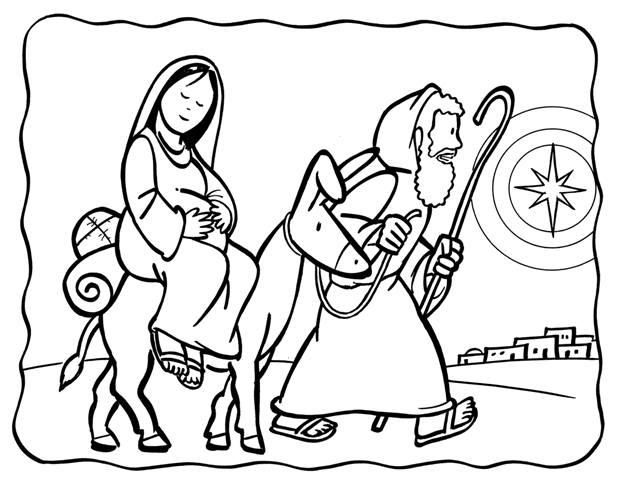
\includegraphics[scale=1]{gambar/11.jpg}
\end{wrapfigure}


\noindent{Adalah utang tetapi mustahil melunasinya namun, merupakan kekayaan dan kenangan paling berharga yang telah memaknai dan mengarisbawahi batin dan hati setiap peziarah ke Tanah Suci yang sampai sekarang masih diperdebatkan oleh Palestina dan Israel. }

Adalah satu pengalaman yang sulit untuk dilupakannya. Pengalaman pribadiku membisikan ketidakpercayaan bahwa suatu saat aku akan mengunjungi Tanah Suci. Aku tidak pernah memimpikannya, apalagi mengharapkan dan merencanakan untuk mengunjunginya. Namun Allah sendiri telah merencanakan sesuatu yang sama sekali berlainan dengan rencanaku. Oleh karena rahmat dan pengutusanNya, aku berhutang padaNya. Apa yang semestinya aku lakukan? Meskipun aku berniat untuk melakukan sesuatu tindakan bagiNya, tentu masih saja tidak berarti. Namun, setidaknya aku mencoba untuk mengoreskan pengalamanku ini kepada orang lain selagi aku bisa.

Betlehem adalah tempat bersejarah yang paling dekat dengan komunitas salesian di Cremisan yang hanya bisa ditempuh kurang lebih $\frac{1}{4}$ jam dengan kendaraan pribadi atau umum. Biasanya para frater memilih alternatif lain untuk mengapainya yaitu berjalan kaki. Merupakan tempat bersejarah pertama yang aku kunjungi ketika baru pertama kali aku menginjakan kakiku di Tanah Suci. Seseorang bisa saja bertanya, apa emosi anda? Tentu saja lain dari yang lain. Emosi setiap orang adalah subyektif. Percaya atau tidak bukanlah permasalahan kita sekarang. Penting adalah bagaimana seseorang dihadapan pada suatu realitas yang selama ini tersembunyi di bawah kemisterian. Artinya, nama Betlehem hanya menjadi sebuah cerita belaka. Selebihnya aku bukan dihadapan pada sebuah misteri tersembunyi. Aku menyentuhnya dengan tanganku sendiri dan mengawasinya dengan mataku sendiri secara seksama. Dan bagaimana gua ini terpelihara hingga sekarang? Merupakan pertanyaan setiap orang, baik bagi mereka yang telah mengunjunginya ataupun bagi mereka-mereka yang hanya mendengar namanya saja. 

Betlehem, adalah nama yang mengekspresikan misteri kemenangan dalam kemiskinan; kemiskinan Bunda Maria dan Santu Yosep namun, kemiskinan mereka diterangi oleh kemenangan Natal dengan kelahiran sang Terang, Yesus Kristus. Terang itu menerangi semua orang di planet bumi ini, menerangi hati dan budi setiap orang yang mencari Allah, seperti terjadi pada orang-orang Majus dari Timur. Terang itu membawa mereka menemukan Yesus seperti yang mereka masing-masing mengharapkannya. Kehadiran Yesus ini adalah sebagai Allah Pembawa damai bagi para umatNya.

Betlehem, dalam bahasa Yahudi, "Rumah Roti" dan dalam bahasa Arab, "Rumah Daging", terletak di pinggir padang gurun yang dalam Kitab Suci dikenal sebagai EFRATA (artinya yang mengandung buah, yang berbuah); berpenduduk sekitar 40.000 orang, mayoritas orang Arab, baik kristiani maupun Islam.

Betlehem adalah satu daerah yang dirahmati dengan beraneka macam kekayaan. Rumah-rumahnya berbatu putih mengkilat, dikelilingi dengan sekelompok besar kawanan domba, yang menciri-khaskan tradisi setempat; dikelilingi juga oleh lahan dengan tanaman zaitun. Dari kesemuanya ini di hadapan pandangan mata kita bagaikan sebuah palungan alamiah yang indah. 

Pada zaman Yesus, meskipun Yehuda adalah termasuk bagian kekuasaan raja Daud, Betlehem tetaplah merupakan sebuah kota kecil tak dikenal di antara kota-kota lain disekitarnya. Keadaan geografisnya tidak menguntungkan untuk menemukan kembali letak kestrategisannya atau kepolitikkannya. Namun, bagaimanapun juga tidak disangkal nama Betlehem pada saat ini termashyur, dikagumi untuk sepanjang dan segala masa. 

Pada zamannya nabi Mikha, ia memprofesikan kemashyuran kota kecil Betlehem, dengan bernubuat:"Engkau, hai Betlehem Efrata, hai yang terkecil di antara kaum-kaum Yehuda, dari padamu akan bangkit bagiKu seorang yang akan memerintah Israel, yang permulaannya sudah sejak purbakala, sejak dahulu kala" (Mi, 5,1).

Di jantung Basilika yang akrabnya dipanggil Basilika Kelahiran Yesus terdapat gua atau kandang domba kelahiran Yesus. Basilika ini merupakan yang tertua di antara semua basilika atau gereja di dunia. Alasannya sederhana: karena merupakan Basilika pertama di Tanah Suci yang memancarkan gua mistik dimana Yesus dilahirkan. Dan selanjutnya menjadi tempat kudus bagi orang-orang Kristen pertama, dan merupakan pusat penghormatan kekudusan Allah. 

Kesaksian sejarah menceritakan bahwa pada zaman Kaisar Adrianus, sekitar tahun 135 setelah Kristus, ia menghendaki agar menghapuskan dari semua tempat kudus lambang-lambang kesucian Kristiani. Begitupun dengan Yerusalem, dimana ia memerintahkan untuk meratakan puncak Golgota, dengan membangunkannya kembali di atas sebuah bangunan untuk memberi penghormatan kepada para dewa-dewi. Di Betlehem, seperti dikisahkan bahwa Gua kelahiran Yesus ini pada awalnya telah disembunyikan dengan timbunan tanah, dan diatasnya ditanamkan sekelompok tanaman hijau, dimana menjadikan Gua kelahiran Yesus ini menjadi sebuah hutan rimba suci bagi dewa kesuburan.

Namun, keprofananya tidak berlangsung lama. Selang waktu sebelum berakhirnya zaman kepahitan itu, gua kelahiran Yesus digunakannya kembali oleh orang-orang kristiani untuk berdoa, adorasi dan sebagainya.
Dari tahun 215, tradisi mengkisahkan juga bahwa kesaksian filsuf dan teolog Origene menunjukkan bahwa Gua itu merupakan tempat kelahiran Penyelamat dunia dan kandang para kawanan domba. Fakta ini membuktikan adanya keaslian. Begitupun sesuai dengan kesaksian orang-orang disekitarnya baik yang percaya maupun yang tidak percaya kepada Allah pada zaman itu.

Pada tahun 325, ibu Kaisar Kostantino, memberikan kepada orang kristen kebebasan untuk beribadat. Maka, Kostantino memulai untuk membangun di atas Gua itu sebuah Basilika. Basilika tertua ini masih terlihat hingga sekarang.

Pada tahun 384, Santo Hieronimus memilih untuk mendirikan di dekat gua ini, sebuah komunitas religius. Orang kudus ini, membaktikan hampir setengah dari hidup kebiaraannya, kurang lebih selama 36 tahun dengan kehidupan berdoa dan menerjemahan Kitab Suci dari bahasa Ibrani dan Yunani ke dalam bahasa Latin; kesaksiannya mengisahkan bahwa: "Hai! Betapa baiknya, seandainya aku dianugerahkan rahmat untuk melihat sendiri keaslian kandang kelahiran dimana Bayi Yesus dilahirkan dan diletakkan! Namun, hanya untuk sebuah venerasi saja, kita telah meniadakan keaslian kandangnya dengan membangunkannya kembali sebuah gua atau kandang berlapiskan marmer. Seberapa harganyakah bagiku semuanya ini? Apa gunanya semuanya ini bagiku?"

Pada tahun 531, Kaisar Yustinianus memperbaikinya lagi bangunan ini yang telah didirikan atas perintah Santa Helena, ibu Kaisar Kostantino. Yustinianus mencoba mengkostruksikannya lagi bangunan ini dengan mempertahankan keasliannya tanpa merubah bentuk keasliannya. Karena bangunan ini telah terukir banyak sejarah, terutama bertahannya terhadap serangan-serangan dari luar seperti dari serangan orang-orang Islam pada umumnya.

Pintu masuk Basilika yang sekarang berukuran sangat kecil; yang tingginya kurang lebih 1 meter dan lebarnya 45 centimeter. Tiga buah pintu lainnya terpaksa ditutup untuk menghindari masuknya para tentara Otomani dengan berkuda. Pintu masuk yang ada hinga sekarang ini sangat rendah ketinggiannya merupakan sebuah kenangan terbaik yang bisa memaknai ingatan budi setiap peziarah. Melambangkan ketidaklayakan manusia di hadapan kemahakuasaan Allah.

\section*{Di gua bersama MARIA}

Tampaknya menjadi sesuatu yang biasa. Bagi siapa yang masuk ke dalam Basilika pertanyaannya yang pertama adalah "dimanakah gua itu"? Gua merupakan pusat dan hati dari basilika. Gua ini dipancarkan dengan sebuah bintang beremaskan perak, dengan tulisan:"di sini, oleh Bunda Maria Yesus dilahirkan". Dengan demikian, pusat perhatian kita di dalam gua itu tertuju pada cahaya tersebut. Para peziarah berlutut dan mencium bintang bersahaja itu. Adalah Misteri cintakasih Allah! Allah dengan bahasa sederhananya, mewahyukan diriNya, menjadikan diriNya visibil, terjangkau, dalam bentuk seorang manusia: "Maria melahirkan seorang anak laki-laki, lalu dibungkusnya sengan lapin dan dibaringkannya di dalam palungan, karena tidak ada tempat bagi mereka di rumah penginapan"(Luk. 2,7). 

Renungkanlah sesaat. Seperti ibu-ibu yang lain, Maria pada saat itu, rupanya sedikit sibuk untuk menamai sang kecil. Maria mulai berbisik kepada sang kecil, tanpa nama itu: "hai bunga kecilku, nama apa yang selayaknya kuberikan untukmu?" Seorang manusia? Tetapi kandunganMu adalah Kudus Ilahi. Engkaukah Tuhan? Tetapi, Engkau mengambil rupa manusia. Jadi, apa yang hendak kuperbuat bagimu? Engkau akan kususui atau dihormati sebagai Yang Kudus, Allah? Akankah kupelihara atau diperlakukan sebagai seorang hamba"?

Ataukah hanya sekedar bahwa pada saat itu, tidak ada tempat penginapan lagi bagi mereka. Ataukah dilahirkan sebagai yang terakhir dari generasi manusia, tanpa rumah pernginapan, tak mempunyai apa-apa. Jawaban yang semestinya diberikan kepadaNya adalah: "Terang itu bercahaya di dalam kegelapan dan orang tidak menerimaNya... Ia datang kepada milik kepunyaanNya, tetapi orang-orang kepunyaanNya itu tidak menerimaNya" (Yoh.1,5-11). 

Pesan Natal, yang seharusnya kita berikan pada setiap perayaan Natal, bukan yang lain selain: "MENERIMA KRISTUS".

Setelah 2000 tahun berlalu, tempat penginapan apa yang kita buatkan untuk Yesus??? Seharusnya kita membuatkan tempat penginapan bagiNya; tempatNya adalah di dalam hati dunia dan hati setiap orang. Karena jika Dia telah menemukan tempat diantara kita dengan cintaNya; dan jika sampai sekarang ini, Dia masih mencari sesuatu dari kita bukan karena Dia menginginkanNya, tetapi demi keselamatan kita, maka seharusnya kita memenuhinya dengan bertumbuh dan lahir dari dalam (hati kita), tanpa harus seseorang yang memanuver, yakni CINTA KASIH.	

Allah (Yesus) telah menjawab "YA" kepada dunia: Manusia seharusnya juga menjawabnya "YA" kepada Allah. Karena itu merupakan satu-satunya kondisi atau jalan untuk memperoleh keselamatan: "tetapi semua orang yang menerimaNya diberiNya kuasa supaya menjadi anak-anak Allah, yaitu mereka yang percaya dalam namaNya"(Yoh.1,12). 

\sumber{Oleh: Fr. Acacio D. De Castro, SDB - Yerusalem \\email: addecastro@yahoo.co.uk}
\normalsize
\newpage
\chap{Kompendium Katekese Gereja Katolik}
\setcounter{kgkcounter}{17}
{\normalsize
\section*{KITAB SUCI}

\kgk{Mengapa Kitab Suci mengajarkan kebenaran?}
Karena Allah sendirilah pengarang Kitab Suci. Atas alasan inilah Kitab Suci
disebut ``terinspirasikan'', dan tanpa kesalahan mengajarkan kebenaran yang per-
          lu untuk keselamatan kita. Roh Kudus menginspirasikan para pengarang yang
          menuliskan apa yang Dia inginkan untuk mengajar kita. Tetapi, iman Kristen
          bukanlah ``agama Kitab'', tetapi agama Sabda Allah – ``bukan kata-kata yang tertulis
          dan bisu, melainkan Sabda yang menjadi manusia dan hidup'' (Santo Bernardus
          dari Clairvaux).

\kgk{Bagaimana Kitab Suci seharusnya dibaca?}
         Kitab Suci harus dibaca dan ditafsirkan dengan bantuan Roh Kudus dan di
  bawah tuntunan Kuasa Mengajar Gereja menurut kriteria: 1) harus dibaca dengan
          memperhatikan isi dan kesatuan dari keseluruhan Kitab Suci, 2) harus dibaca
          dalam Tradisi yang hidup dalam Gereja, 3) harus dibaca dengan memperhatikan
          analogi iman, yaitu harmoni batin yang ada di antara kebenaran-kebenaran iman
          itu sendiri.

\kgk{Apa kanon Kitab Suci itu?}
Kanon Kitab Suci ialah daftar lengkap dari tulisan-tulisan suci yang diakui oleh
Gereja melalui Tradisi Apostolik. Kanon ini terdiri dari 46 kitab Perjanjian Lama
          dan 27 kitab Perjanjian Baru.

\kgk{Apa pentingnya Perjanjian Lama bagi umat Kristen?}
Para pengikut Kristus menghormati Perjanjian Lama sebagai Sabda Allah
          yang benar. Seluruh Kitab Perjanjian Lama itu diinspirasikan secara ilahi dan
          mempunyai nilai tetap. Kitab-kitab itu memberikan kesaksian tentang pedagogi
          ilahi cinta Allah yang menyelamatkan. Kitab-kitab itu ditulis terutama untuk
          mempersiapkan kedatangan Kristus sang Penyelamat alam semesta.


\flushright{(\dots \emph{bersambung} \dots)}
}
\end{document}